\newcounter{nuserstory}

\newcommand{\userstory}[4]{%
    \refstepcounter{nuserstory}
    \subsection{#1}
    \label{userstory:\thenuserstory}
    \hangindent=40pt
    \textbf{\textit{As a}} #2,\\
    \textbf{\textit{I want to}} #3,\\
    \textbf{\textit{so that}} #4.
}


\chapter{Requirement Analysis}
\label{chap:requirement-analysis}

\section{Stakeholder Analysis}
\label{section:stakeholder-analysis}
\subsection{Primary Stakeholders}
\label{subsection:primary-stakeholders}

\begin{enumerate}[leftmargin=80pt]
    \item \textbf{Users:} Users represent the target users of our application. They often struggle to find parking, and our app helps by providing parking availability information. For specification of our users see \ref{section:target-user}.
    \item \textbf{Parking Area Owners:} Parking area owners are people or organizations that manage parking facilities around the campus. Due to financial constraints, their options for utilizing the parking area are limited, but they still want to provide availability information for visitors. They play a key role as site owners, controlling the existing infrastructure within the system.
\end{enumerate}

\section{User Stories}
\label{section:user-stories}

\userstory{Parking Availability Indicator% 
}{driver on Kasetsart University campus% 
}{see the parking availability indicator% 
}{I don't waste time driving to all parking areas}

\userstory{Navigation to Available Parking% 
}{visiting driver looking for parking% 
}{be guided directly to available parking areas% 
}{I can efficiently reach parking without unnecessary detours}

\userstory{Destination-based Parking Search% 
}{campus visitor% 
}{specify my destination and see nearby parking options with availability status% 
}{I can choose the most convenient parking location for my needs}

\userstory{Existing Infrastructure Utilization% 
}{parking area owner% 
}{implement a parking availability indicator system using existing infrastructure% 
}{I can provide parking information to visitor without significant investment}

\userstory{Lightweight On-Site Resources Requirements% 
}{parking area administrator% 
}{deploy a solution that doesn't require high computing performance on-site% 
}{I can implement the system with existing resources and minimal operating costs}

\section{Use Case Diagram}
\label{section:use-case-diagram}
<TIP: Write a use case diagram for your project here. Refer to an
article “What is a use case diagram?” by Lucidchart for help./>

\section{Use Case Model}
\label{section:use-case-model}
A use case is a detailed description of how a system
interacts with an external entity (such as a user or another system) to
accomplish a specific goal. Use cases provide a high-level view of the
functionality of a system and help in capturing and documenting its
requirements from the perspective of end users.

<TIP: Write use cases for your project here. Make sure to use the
appropriate type of use case for each scenario (brief, casual, and fully-dressed
use case)./>

\section{User Interface Design}
\label{section:user-interface-design}
The user interface of KU Parking emphasizes usability and mobile compatibility. It includes familiar components commonly found in map applications, prioritizing the reduction of the learning curve and allowing users to navigate the app.

\begin{figure}[h]
    \centering
    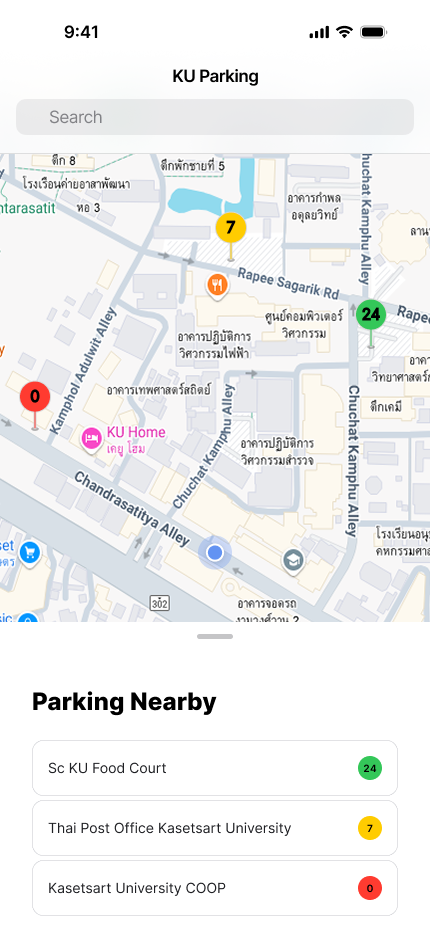
\includegraphics[width=0.5\textwidth]{ui-design/parking-indication.png}
    \caption{User Interface Design for Parking Indication}
\end{figure}

\begin{figure}[h]
    \centering
    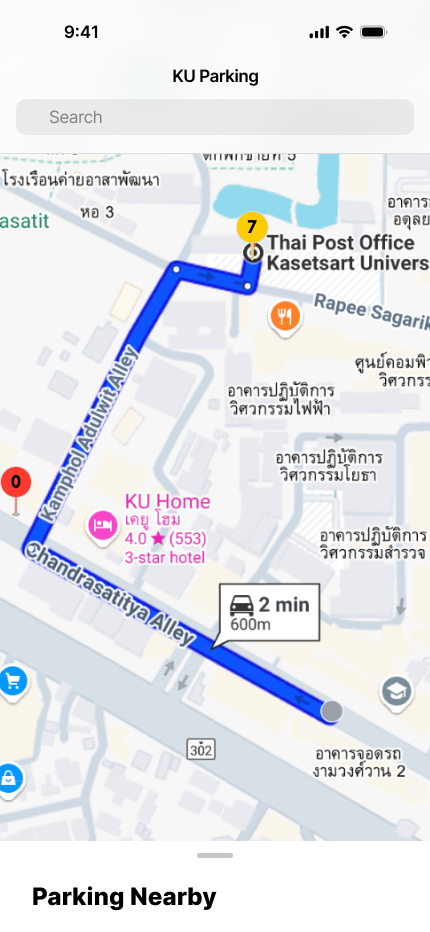
\includegraphics[width=0.5\textwidth]{ui-design/navigation.png}
    \caption{User Interface Design for Navigation}
\end{figure}